\documentclass{article}

\usepackage{amsmath}
\usepackage{amssymb}
\usepackage{parskip}
\usepackage{fullpage}
\usepackage{hyperref}
\usepackage{tikz}

\hypersetup{
    colorlinks=true,
    linkcolor=black,
    urlcolor=blue,
    pdftitle={Limits},
    pdfpagemode=FullScreen,
}

\title{Limits}
\author{Paolo Bettelini}
\date{}

\begin{document}

\maketitle
\tableofcontents
\pagebreak

\section{Definition}

A limit is usually used to describe the behavior of a function as its argument approaches a given value.
The limit towards a certain value \(c\) within a function can be be approached both from the right and from the left.
The limit in a general sense exists if the value approached from both sides is the same and well-defined.
We define the limit of \(x\) approaching \(c\) from the left within the function \(f(x)\) as
\[
    \lim_{x\to c^{-}}f(x)
\]
We define the limit of \(x\) approaching \(c\) from the right within function \(f(x)\) as
\[
    \lim_{x\to c^{+}}f(x)
\]
We define the limit of \(x\) approaching \(c\) within function \(f(x)\) as
\[
    \lim_{x\to c}f(x)
\]

Formally, given a function \(f:D\to \mathbb{R}\) the limit \(L=\lim_{x\to c}f(x)\) exists if given an arbitrary small \(\epsilon >0\) there is another number \(\delta >0\) such that
\[
    |f(x)-L|<\epsilon
    \text{ when }
    0<|x-c|<\delta
\]

\begin{center}
    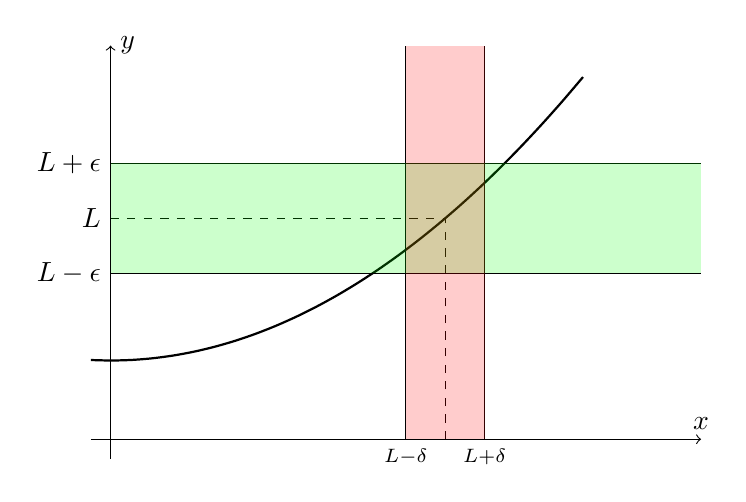
\begin{tikzpicture}[
        declare function={
            func(\x) = \x*\x / 10 + 1;
            LimX=4.25;
            Epsilon=0.7;
            Delta=0.5;
            LimY={func(LimX)};
            Width=7.5;
            Height=5;
        }
    ]
        \draw[->] (0, -0.25) -- (0, Height) node[right] {\(y\)};
        \draw[->] (-0.25, 0) -- (Width, 0) node[above] {\(x\)};

        \draw[domain=-0.25:6, smooth, variable=\x, black, thick] plot ({\x}, {func(\x)});

        \draw[-, dashed] (LimX, 0) -- (LimX, LimY);
        \draw[-, dashed] (0, LimY) node[left] {\(L\)} -- (LimX, LimY);

        \draw[-] (0, {LimY + Epsilon}) node[left] {\(L + \epsilon\)} -- (Width, {LimY + Epsilon});
        \draw[-] (0, {LimY - Epsilon}) node[left] {\(L - \epsilon\)} -- (Width, {LimY - Epsilon});

        \draw[-] ({LimX - Delta}, 0) node[below] {\(\scriptstyle L - \delta\)} -- ({LimX - Delta}, Height);
        \draw[-] ({LimX + Delta}, 0) node[below] {\(\scriptstyle L + \delta\)} -- ({LimX + Delta}, Height);

        \fill [green, opacity=0.2] (0,{LimY - Epsilon}) rectangle (Width, {LimY + Epsilon});
        \fill [red, opacity=0.2] ({LimX - Delta}, 0) rectangle ({LimX + Delta}, Height);
    \end{tikzpicture}
\end{center}

This means that for any \(x\) in the red region \(0<|x-c|<\delta\text{ or }|x-c|\in (0; \delta)\),
the function at that point will lie in the yellow region.
This value is closer to \(L\) than either \(L + \epsilon\) or \(L - \epsilon\)
\[
    |f(x) - L| < \epsilon
\]
Notice that this defintion does not require \(f\) to be defined at \(c\), but rather just around \(c\).

We can also use this definition for limits from the right and from the left.

The right-hand limit \(L=\lim_{x\to c^{+}}f(x)\) exists if for any arbitrary small \(\epsilon > 0\)
there is some \(\delta > 0\) such that
\[
    |f(x)-L|<\epsilon \text{ when } 0 < x-c < \delta
\]

The left-hand limit \(L=\lim_{x\to c^{-}}f(x)\) exists if for any arbitrary small \(\epsilon > 0\)
there is some \(\delta > 0\) such that
\[
    |f(x)-L|<\epsilon \text{ when } -\delta < x-c < 0
\]

\pagebreak

\section{Properties}

If the limit exists
\[
    \lim_{x\to c}f(g(x))=f(\lim_{x\to c}g(x))
\]

\section{Continuity}

A function \(f\) is continuous at a point \(c\) iff
\[
    \lim_{c_0 \to c^+} f(c_0) = \lim_{c_0 \to c^-} f(c_0) = f(c)
\]
A function \(f\) is continuous on an interval \([a;b]\) iff it is continuous at each point \(c \in [a;b]\)
\[
    \forall c \in [a;b],
    \lim_{c_0 \to c^+} f(c_0) = \lim_{c_0 \to c^-} f(c_0) = f(c)
\]

\section{Intermediate value theorem}

A function \(f\) continuous on an interval \([a;b]\) will take
every value in the interval \([f(a);f(b)]\).

\pagebreak

\section{Bolzano's Theorem}

If \(f(x)\) is continuous on \([a;b]\) and \(f(a)<f(b)\) then there is a root.
\[
    f(a)<f(b) \implies \exists c \in [a;b] \mid f(c) = 0
\]

\section{Squeeze Theorem}

Let \(h(x)\), \(f(x)\) and \(g(x)\) be three functions such that
\(h(x) \leq f(x) \leq g(x)\). \\
If
\[
    \lim_{x \to x_0} g(x) = f(x) = L
\]
then
\[
    \lim_{x \to x_0} f(x) = L
\]

% https://raw.githubusercontent.com/MassimilianoCEZ/Math/main/IT/3rd_year/Analisi_1/ripasso.pdf

\end{document}
